\section{Experiments and results}\label{chapter4}

\subsection{Dataset}

Our neural network is designed to classify $10,000$ unlabelled samples with $128$ features and $10$ different classes, using $60,000$ similar labelled samples. As described in Section~\ref{sec:early}, we split the labelled dataset into $50,000$ training samples and $10,000$ CV samples. The features in the dataset range from $-2045.92$ to $2803.84$ (Figure~\ref{fig:freq-hist}).
\begin{figure}
	\centering{
	%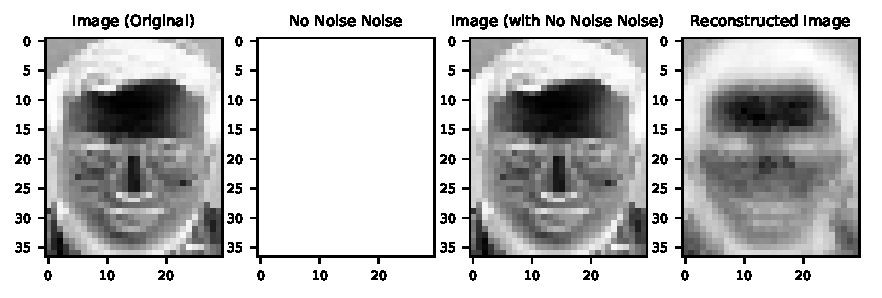
\includegraphics[scale=.9]{Result_Multiplication_KL_Divergence_No_Noise_Comparison}
	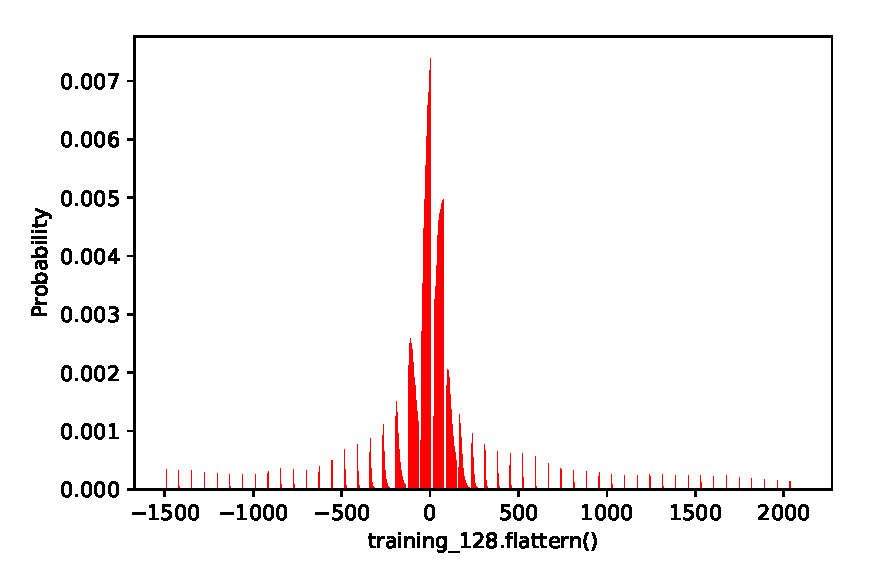
\includegraphics[scale=0.8]
    {resource/hist.eps}}
    \caption{The frequency plot of our training input dataset. Most features of samples are within the range~$(-300,300)$. However, features can be as large as $2803.84$ or as small as $-2045.92$.}
    \label{fig:freq-hist}
\end{figure}

%Then we use all the $60,000$ samples to build our final neural network model.
\subsection{Use Numpy and Scipy for code vectorisation}
We use \texttt{python} 3.6 to code the neural network model with a list of library dependencies specified in the file named \texttt{requirements.txt} file in our git repository. 
In particular, our model requires the scientific computing library \texttt{scipy 1.21}, and uses \texttt{numpy} to perform vectorised matrix algebra operations.

\subsection{Multiprocessing speeds up hyperparameters tuning}
%We apply three layers neural network model with three different activation functions such as tanh, sigmoid and ReLu for the hidden layers as well as a Softmax activation function for the output layer.
%We apply batch normalisation to the input for each layer to reduce the training time and make our model more resilient to parameter scale.
%As for the regularisation techniques,
%we use early stopping, drop out and weight decay to prevent over-fitting.
%We use combinations of all the above setups to tune the hyperparameters for our neural network model,
%in the end we successfully find the benchmark model to use for prediction with best accuracy and reasonable runtime.
Column~1 in Table~\ref{table:best-four-steps} illustrates the hyperparameters of our Benchmark neural network, which completes the classification task with a CV accuracy of $89.9\%$ within $2.3$ minutes.

To demonstrate the effect of each module in the benchmark model, we perform one way sensitivity analysis by varying one selected module in each experiment. 
In the five experiments shown in Table~\ref{tb:comp}, we turn up the drop out rate from $0.05$ to $0.5$, turn the momentum coefficient from $0.9$ to $0$, turn weight decay coefficient from $0.0007$ to $0$, replace mini-batch training by batch training, and train the model without BN, respectively.
\begin{table}
\caption{Hyperparameters for models which output outstanding CV accuracy. The benchmark model is our best model in terms of accuracy as well as speed. Hyperparameter sets~$2$--$5$ are either slightly less accurate or slower than our benchmark model. The row of running time is the time taken to train our neural network and make prediction with the computer detailed in Figure~\ref{fig:hardware}. The row of CV accuracy reports the classification accuracy of the CV samples, which includes the generalisation error and hence approximates the test accuracy. The row of initialisation states the supports of the uniform distribution in initialisation. The method of `Xavier' is introduced in Section~\ref{sec:xav}. The row `Optimal epoch' states the number of epoch corresponding to the highest CV accuracy when training our model (Section~\ref{sec:early}). \label{table:best-four-steps}}
\centering
{
\begin{tabular}{@{}lrrrrr@{}}
\toprule
Hyperparameters                & Benchmark  & Run 2           & Run 3           & Run 4  & Run 5  \\ \midrule
Run time (minutes)             & 2.3     & 2.7              & 3.6              & 17.2    & 10.8    \\
CV Accurarcy                 & 89.9\%  & 89.7\%           & 89.8\%           & 90.0\%  & 89.3\%  \\ \midrule
Initialisation            & Xavier  & \parbox[t]{1.3cm}{\raggedleft Uniform\\$(-1,1)$} 
& \parbox[t]{1.3cm}{\raggedleft Uniform\\$(-1,1)$} 
                                                                            & Xavier  & Xavier  \\
Batch size                & 1500    & 1500             & 1500             & 1500    & 1500    \\
Nodes per layer         & 160     & 150              & 150              & 900     & 160     \\
Activation function       & $\tanh$ & $\tanh$          & $\tanh$          & $\tanh$ & sigmoid \\
Weight decay rate         & 0.0007  & 0.0007           & 0.0007           & 0.0007   & 0.0007   \\
Momentum rate             & 0.9     & 0.9              & 0.92             & 0.9     & 0.9     \\
dropout rate              & 0.05    &0              & 0              & 0.5     & 0.05    \\
Learning rate             & 0.11    & 0.05             & 0.05             & 0.11    & 0.11    \\
Optimal epoch & 44      & 54               & 66               & 158     & 282     \\ 
BN & True      & True          & True          & True       & True          \\\bottomrule
\end{tabular}
}
\end{table}
\begin{table}
\caption{The accuracy of our benchmark model with one selected module either turned off or modified. The row of running time is the time taken to train our neural network and make predictions with the computer detailed in Figure~\ref{fig:hardware}. The row of CV accuracy reports the classification accuracy of the CV samples, which includes the generalisation error and hence approximates the test accuracy. The row of initialisation states the supports of the uniform distribution in initialisation. The method of `Xavier' is introduced in Section~\ref{sec:xav}. The row `Optimal epoch' states the number of epoch corresponding to the highest CV accuracy when training our model~(Section~\ref{sec:early}).
\label{tb:comp}}
\centering
{\centering
\begin{tabular}{@{}lrrrrrr@{}}
\toprule
Hyperparameters             & {\parbox[t]{1.4cm}{\raggedleft Drop \\out 50\%}  } 
& Momentum & {\parbox[t]{1.3cm}{\raggedleft Weight \\decay}} & {\parbox[t]{1.3cm}{\raggedleft Mini-\\batch}} & BN \\ \midrule
Run time (mins)             & 0.5        & 8.6          & 0.8      & 7.6 & 4.5          \\
CV Accurarcy                   & 85.5\%     & 89.4\%       & 88.6\%   & 87.5\% &82.8\%       \\ \midrule
Initialisation              & Xavier     & Xavier       & Xavier   & Xavier & Xavier        \\
Batch size                   & 1500       & 1500         & 1500     & 50000    & 1500        \\
Nodes per layer        & 160        & 160          & 160      & 160    & 160         \\
Activation function        & $\tanh$    & $\tanh$      & $\tanh$  & $\tanh$  & $\tanh$       \\
Weight decay rate          & 0.0007     & 0.0007       & 0        & 0.0007  & 0.0007        \\
Momentum rate                & 0.9        & 0            & 0.9      & 0.9    & 0.9         \\
Dropout rate                & 0.5        & 0.05         & 0.05     & 0.05    & 0.05        \\
Learning rate                & 0.11       & 0.11         & 0.11     & 0.11    & 0.11       \\
Optimal epoch       & 9          & 198          & 16       & 177     & 80       \\ 
BN       & True          & True          & True       & True     & False       \\ \bottomrule
\end{tabular}
}
\end{table}

We implement a \texttt{shell} script to run all these tests in parallel in a high performance computer, whose hardware specification is shown in Figure~\ref{fig:hardware}. The \texttt{shell} script trains our model with various hyperparameters from different 
\texttt{json} files in parallel. 
Running multiple experiments in parallel allows us to fully utilise our computing resources, and tune hyperparameters efficiently. Although the speed for each task has been dropped by $30\%$, this parallel setting dramatically reduces the total running time required to finish the ten experiments detailed in Tables~\ref{table:best-four-steps} and~\ref{tb:comp}. For example, fitting our neural networks with these ten different sets of hyperparameters in parallel takes $17.2$ minutes, which actually equals the time required by the largest model in  Table~\ref{table:best-four-steps}. However, fitting the ten neural networks in sequence takes a total of $44$ minutes, which doubles the total time required in the parallel setting.
\begin{figure}
    \center{
        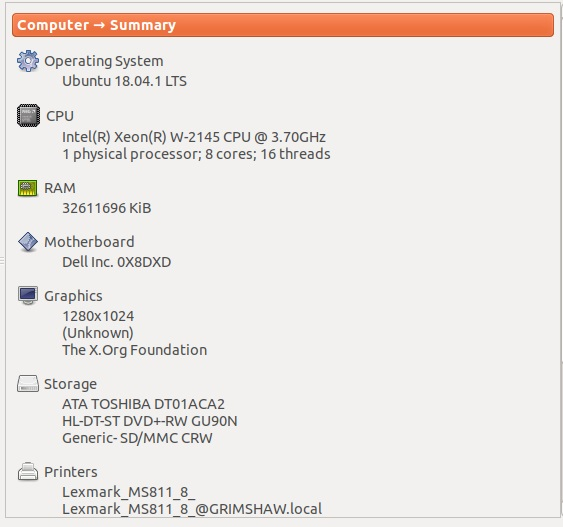
\includegraphics[scale=0.7]{resource/hardware.png}
    }
    \caption{The hardware specification of our high performance computer.}
    \label{fig:hardware}
\end{figure}
\subsection{Experiments Results}
\subsubsection{Early stopping decides optimal number of epochs}
%Early stopping is a form of regularisation technique we use to avoid over-fitting for our neutral network,
%it guides us on how many iterations can be run before the model begins to over-fit.
For the benchmark model listed in Table~\ref{table:best-four-steps}, early stopping detailed in Section~\ref{sec:early} finds $44$ epochs give the best CV accuracy, which is $89.9\%$ (Figure~\ref{fig:acc-iter}). As a result, we choose $44$ epochs as our early stopping point for the benchmark model. By back propagation, we iteratively find the weight matrices~$w_1,w_2,w_3$ as shown in Figure~\ref{fig:weight}.
\begin{figure}
    \center{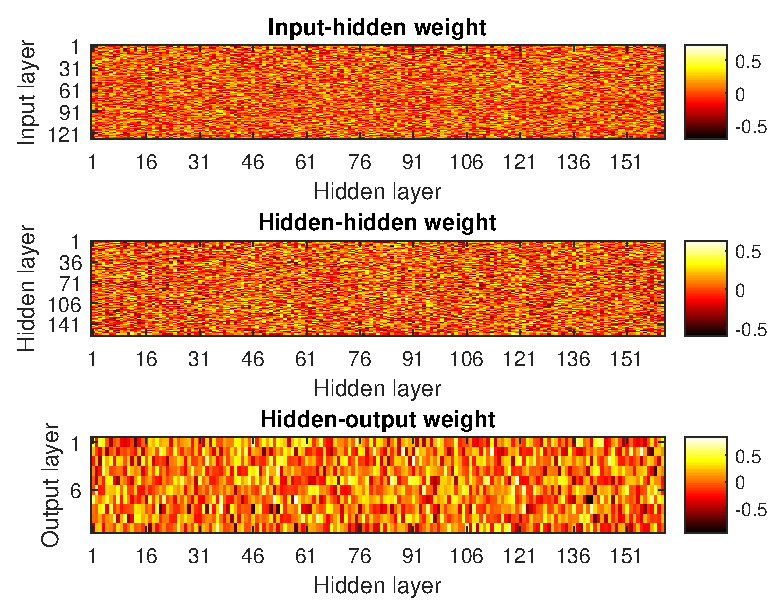
\includegraphics
    {resource/figure2.eps}}
    \caption{\label{fig:weight} A visualisation of the optimal weight matrices for our benchmark model.}
\end{figure}
% shows that the cross validation accuracy of our benchmark model reaches a maximum (89.6\%) has at the $44$th iteration. After then, ...
\begin{figure}
	\centering{
	%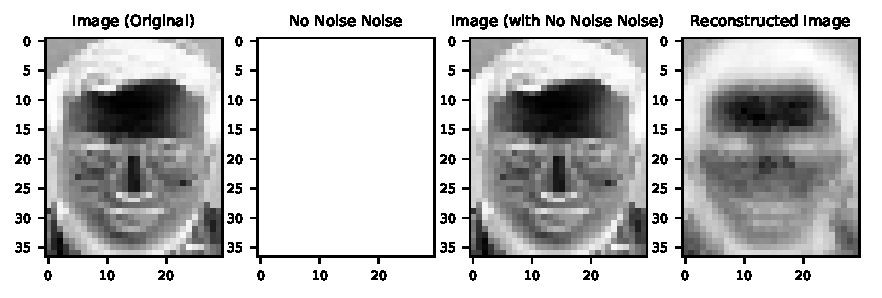
\includegraphics[scale=.9]{Result_Multiplication_KL_Divergence_No_Noise_Comparison}
	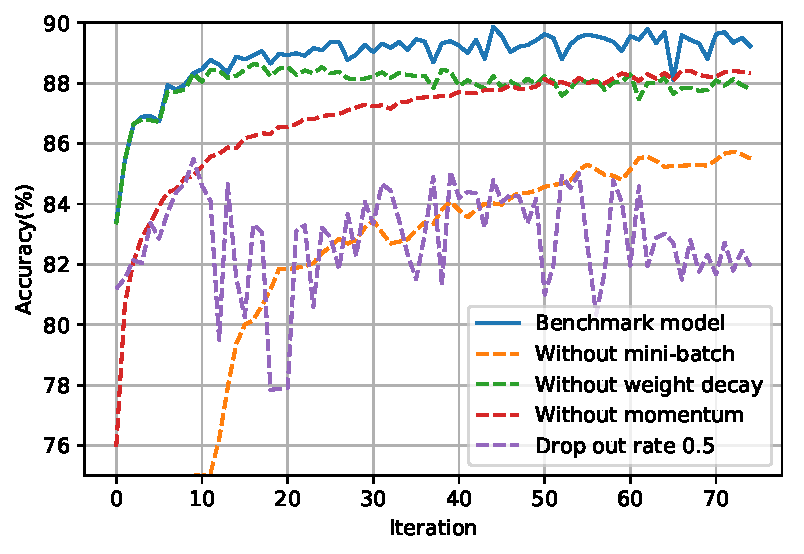
\includegraphics[trim={0 0.2cm 0 0},clip]{data/cost-graph/acc}}
    \caption{The cross plots the training accuracy of our benchmark model, and the  solids line plots the CV accuracy. The dashed lines plots the CV accuracy of modified benchmark models where exact one hyperparameter is modified from the benchmark model.}
    \label{fig:acc-iter}
\end{figure}
\subsubsection{Optimal hyperparameters}
In terms of accuracy and training speed, our best neural network model is the `benchmark' model detailed in Table~\ref{table:best-four-steps}. Although the CV accuracy of the benchmark model is $0.1\%$ lower than the $4th$ hyperparameter who has $900$ nodes in each hidden densely connected layers, it is $8$ times faster. As a result, it is selected as our benchmark model. Table~\ref{tb:comp} and Figure~\ref{fig:acc-iter} illustrate the impact of drop out, momentum, weight decay, mini-batch and BN, respectively, in the Benchmark model.

\subsubsection{Dropout helps in large neural networks}
In the benchmark model, turning up the drop out rate from $5\%$ to $50\%$ not only makes the model less accurate (Table~\ref{tb:comp}), but also makes thw CV accuracy volatile (Figure~\ref{fig:acc-iter}). However, with the $50\%$ drop out rate, the largest neural network model with $900$ nodes per hidden layer turns out to be our most accurate model, which has a CV accuracy of $90\%$ (Table~\ref{table:best-four-steps}). 

\subsubsection{Momentum and mini-batch speed up the convergence}
When turning off the momentum, column~2 in Table~\ref{tb:comp} shows that the time required to train the neural network model suddenly increases from $2.3$ minutes (Benchmark model) to $8.6$ minutes. This is also demonstrated in Figure~\ref{fig:acc-iter}. Moreover, comparing column~2 and~3 in Table~\ref{table:best-four-steps}, it seems that  training sometimes is slower if the momentum coefficient is set to be too high.

In comparison with mini-batch training, batch training has a much longer training time  (Column~4 in Table~\ref{tb:comp}). The longer training time is caused by the slowness of large matrix multiplication in gradient descent.

\subsubsection{Weight decay prevents over-fitting}
Column~3 in Table~\ref{tb:comp} demonstrates that weight decay improves our model performance. As shown in Figure~\ref{fig:acc-iter}, the overfit when training neural network without weight decay drives the purple dashed line to decreases after epoch~$14$. In comparison, the orange solid line, which is the CV accuracy of our benchmark model with weight decay, oscillates after epoch~$44$, without a trend of decline.


\subsubsection{BN significantly improves the accuracy}
In terms of accuracy, BN is the most important module in our neural network model. Turning off BN in our model decreases the CV accuracy from $89.9\%$ to $82.8\%$.


\subsubsection{Sigmoid is slower than tanh}
We attempt to use the sigmoid activation function to replace the $\tanh$ function in the first densely connected layer. As shown at Column~5 in Table~\ref{table:best-four-steps}, this makes our model converges five times slower. Hence we choose $\tanh$ as the activation function in the benchmark model.
% After 44 iter, the cross validation is almost same, but training acc still going up - overfit
% No weight decay - going down
% no momentum - slow
% Dropout rate 
% without mini batch - slow





% \begin{figure}
%     \center{\includegraphics
%     {resource/acc.eps}}
%     \caption{\label{fig:my-label2}Results and parameters of different setups for 89.87 results.}
% \end{figure}